\parindent=0em
\section{Definición}
\noindent

%\footnote{https://www.apple.com/augmented-reality/}

Para poder comprender la tecnología de realidad mixta es necesario conocer los conceptos de realidad aumentada y realidad virtual. La realidad aumentada~\cite{ardefinition} es una tecnología mediante la cual el usuario visualiza el mundo real con el añadido de que puede ver objetos ``sobreimpresionados'', es decir, elementos superpuestos al mundo real.(figura~\ref{fig:ikeaAR}).

\begin{figure}[H]
    \centering
    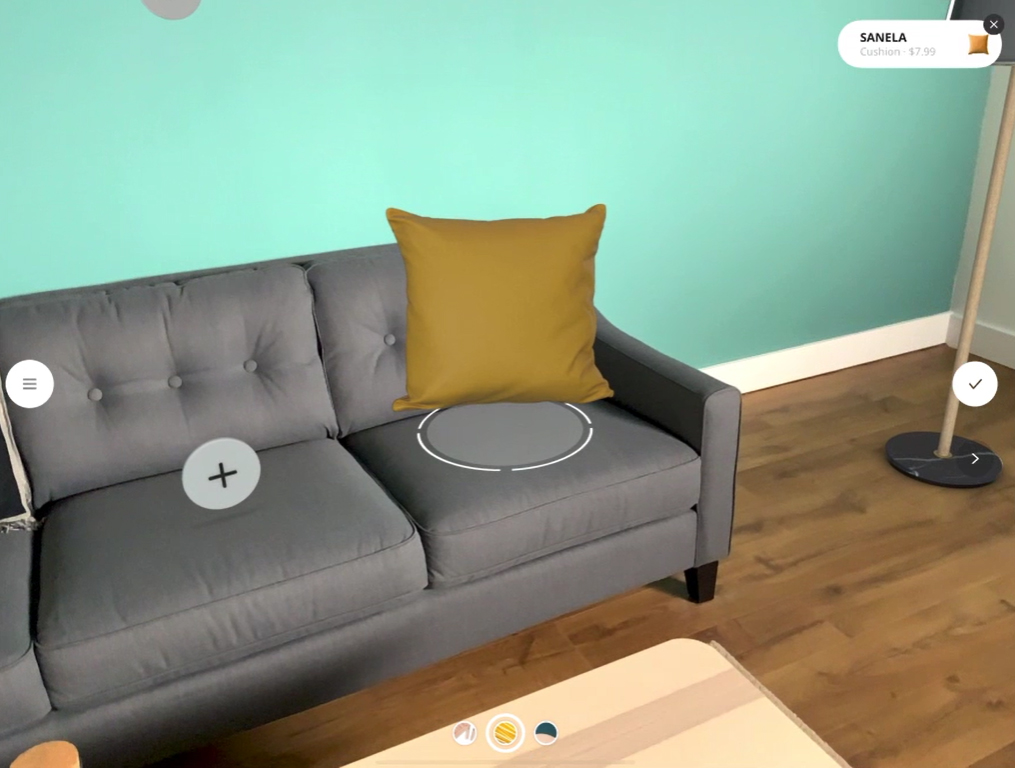
\includegraphics[scale=0.25]{Images/Estado del arte/ikeaAR.jpg}
    \caption[Aplicación de Apple IKEA Place]{Aplicación de Apple IKEA Place\footnotemark.}
    \label{fig:ikeaAR}
\end{figure}
\footnotetext{Fuente: \url{https://www.apple.com/augmented-reality/}}

En la realidad aumentada o AR (del inglés \textit{Augmented Reality}) los elementos creados por ordenador que se colocan en el mundo real no tienen conocimiento de los elementos que existen en el entorno donde se están posicionando. \\

Existen dos tipos de realidad aumentada~\cite{arwithMarkers}, realidad aumentada con marcadores y realidad aumentada sin marcadores. Los marcadores son imágenes en 2D con símbolos o características especiales que son fáciles de captar (figura~\ref{fig:armaerkersexample}), estos marcadores son usados en la realidad aumentada con marcadores para colocar los objetos virtuales. En cambio, la realidad aumentada sin marcadores utiliza distintos sensores para obtener la información que aporta un marcador.

\begin{figure}[H]
    \centering
    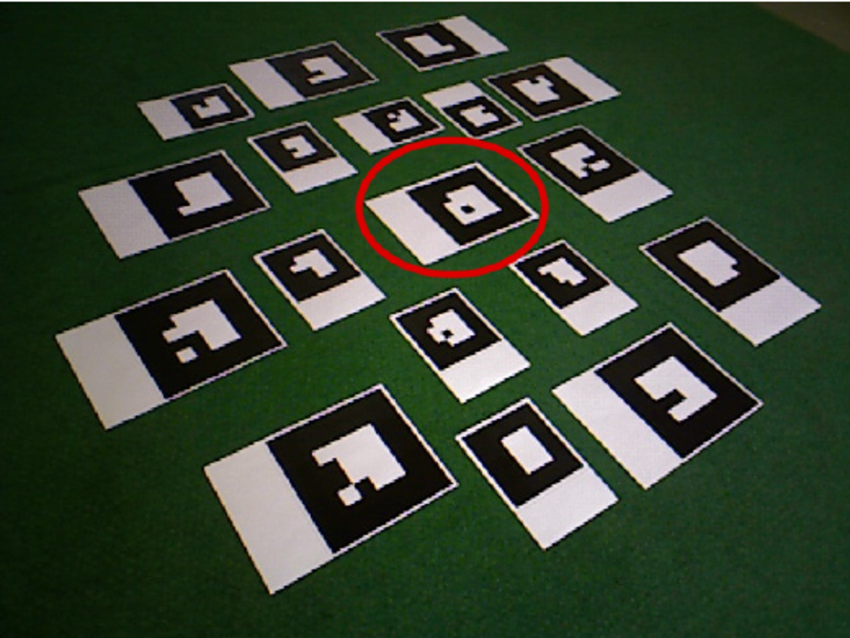
\includegraphics[scale=0.25]{Images/Estado del arte/armarkers.png}
    \caption{Ejemplo de marcadores de AR~\cite{arMarkerArticle}.}
    \label{fig:armaerkersexample}
\end{figure}

Por otro lado, la realidad virtual~\cite{vrintroduction} o VR (del inglés \textit{Virtual Reality}) es una tecnología basada en la simulación de un entorno generado por ordenador que destaca por ser una experiencia inmersiva completa (figura~\ref{fig:superhotVR}). Esto se consigue gracias a la sensación de presencia en el entorno virtual que se genera en el usuario principalmente a través del sentido de la vista y del sonido. En la realidad virtual el usuario se coloca un dispositivo con el que no puede ver nada del mundo físico.

\begin{figure}[H]
    \centering
    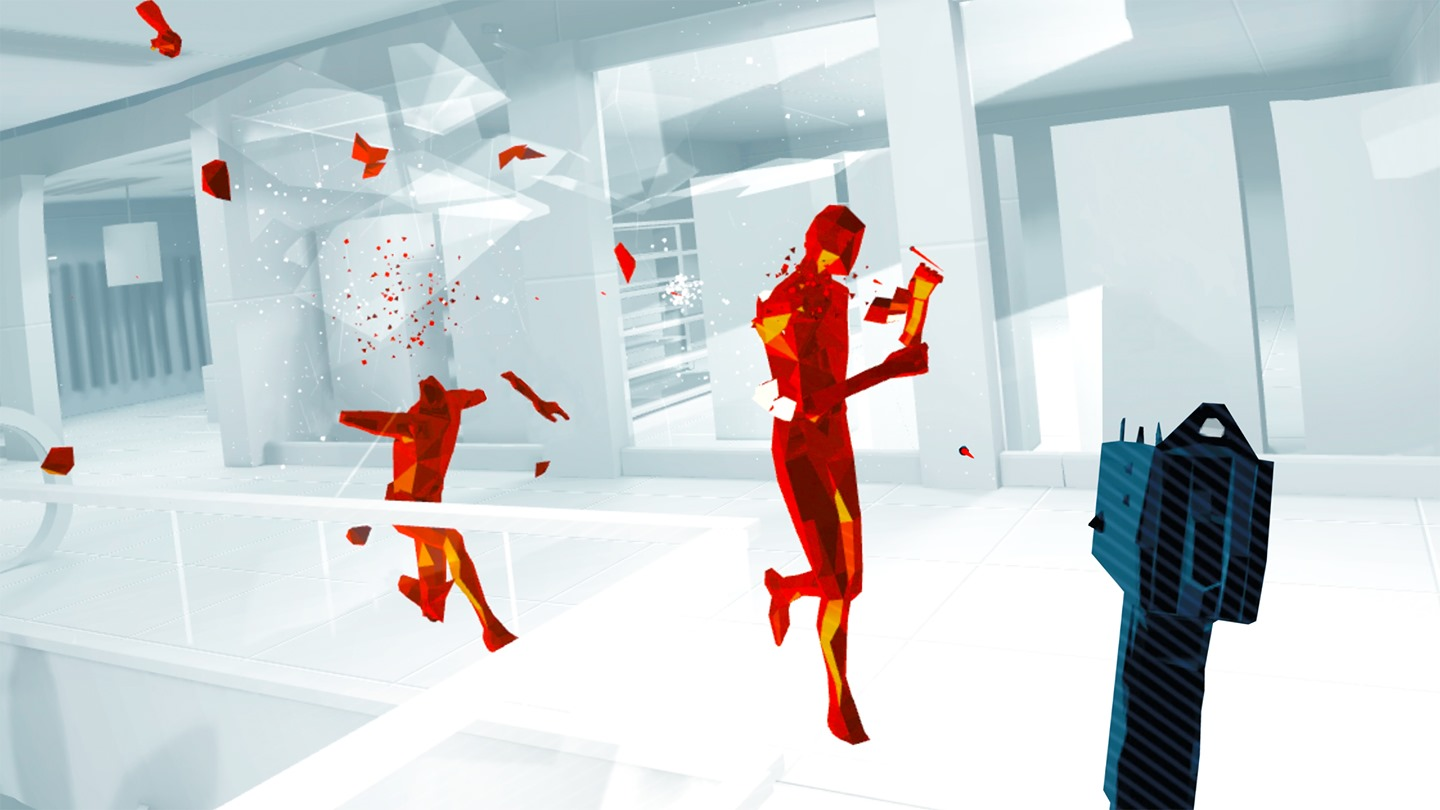
\includegraphics[scale=0.25]{Images/Estado del arte/superhotvr.jpg}
    \caption[Captura del juego de realidad virtual SUPERHOT VR.]{Captura del juego de realidad virtual SUPERHOT VR\footnotemark. El usuario maneja el arma con el que dispara a los enemigos de color rojo.}
    \label{fig:superhotVR}
\end{figure}
\footnotetext{Fuente: \url{https://www.oculus.com/experiences/quest/1921533091289407/}}
A diferencia de la realidad aumentada, en la realidad virtual todos los elementos son conscientes de la existencia de los otros objetos, ya que todo el entorno pertenece a la misma simulación y el mundo real no participa en ella.\\

%superhotVR https://www.oculus.com/experiences/quest/1921533091289407/


Por otra parte, se conoce como realidad mixta o MR (del inglés \textit{Mixed Reality}) a la combinación de realidad virtual y realidad aumentada, es decir, a la fusión de la interacción entre elementos físicos y virtuales (figura~\ref{fig:mrdefinitionexample}). En esta tecnología el usuario está presente en un mundo que es tanto virtual como físico, destacando principalmente la posibilidad de interacción de los objetos con el entorno.\\

\begin{figure}[H]
    \centering
    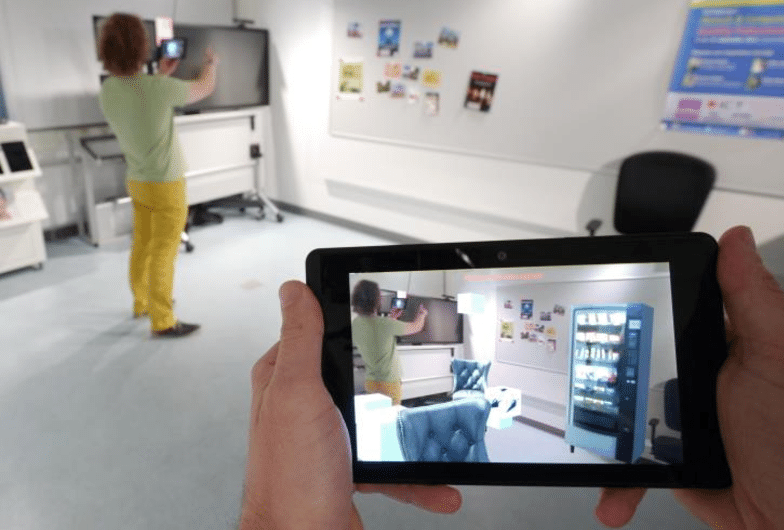
\includegraphics[scale=0.3]{Images/Estado del arte/mrexampledefinition.png}
    \caption{Experiencia colaborativa de MR con dos tabletas~\cite{mrExampleDefinition}. En la tableta se puede ver como se están mostrando elementos virtuales que no existen en el mundo físico mientras la otra persona interactúa con otros elementos de la pared.}
    \label{fig:mrdefinitionexample}
\end{figure}

Fue en 1994 cuando Paul Milgram y Fumio Kishino definieron el concepto del continuo de la virtualización~\cite{ARDisplayofContinuum}, indicando que la realidad mixta se define como el entorno que se encuentra en cualquier punto entre los extremos de éste, es decir, entre la realidad aumentada y la realidad virtual (figura~\ref{fig:rvcontinuumfig}).\\


Por último, se conoce con el término de realidad extendida~\cite{xrintro} o XR (del inglés \textit{eXtended Reality}) a la tecnología que abarca el conjunto de las tres realidades mencionadas anteriormente, realidad aumentada, realidad mixta y realidad virtual.  

\begin{figure}[htbp]
\centering
    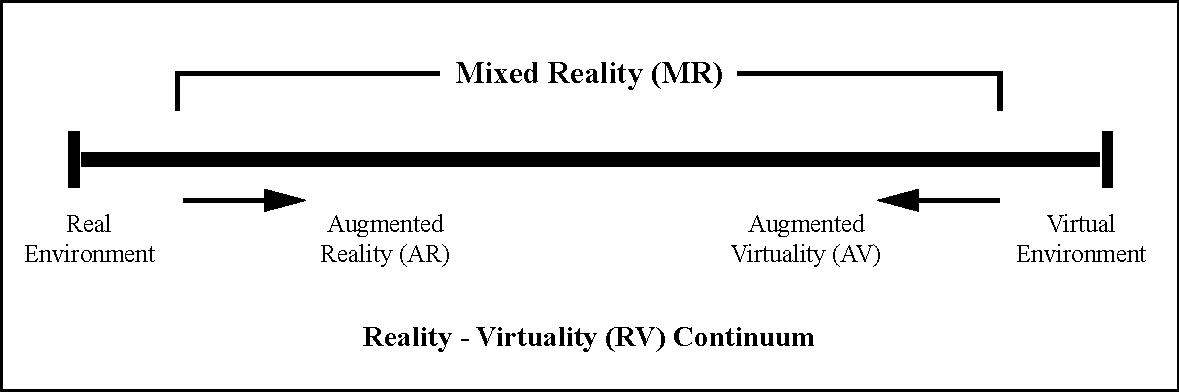
\includegraphics[scale=0.7]{Images/Estado del arte/rvcontinuum.pdf}
    \caption{Reality-Virtualiy Continuum \cite{ARDisplayofContinuum}.}
    \label{fig:rvcontinuumfig}
\end{figure}






